

\section{Compiling NVIDIA Jetson Linux with PPS}
\begin{figure}[H]
    \centering
    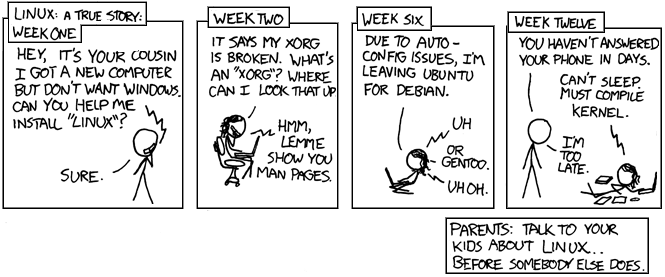
\includegraphics[width=\textwidth]{figures/cautionary.png}
    \caption{Cautionary by XKCD \cite{xkcdCautionary2008}}
    \label{fig:xkcd_cautionary}
\end{figure}
\subsection{Background}
\gls{pps} is a high precision signal that repeats every seconds provided by a device, typically a GPS receiver, that is used to adjust the system clock time with high accuracy \cite{giomettiLinuxPPSWikiLinuxPPS2007}.
The \gls{pps} signal is often used in combination with \gls{ntpd} to synchronize the system clock with to \gls{utc} with sub millisecond accuracy \cite{giomettiLinuxPPSWikiLinuxPPS2007}.
As \gls{pps} interrupts are hardware based it appears necessary to configure the Linux Kernel as it is responsible for handling interrupts \cite{giomettiLinuxPPSWikiLinuxPPS2007}.
The kernel is the core software component of an operating system that manages system resources and provides a bridge between software applications and hardware devices as visuzlized in Figure \ref{fig:kernel_visualization} \cite{thekerneldevelopmentcommunityInterruptsLinuxKernel}.
On the \sr a \gls{pps} signal from one of the \glsps{f9p} is used to sunchronize the clock on the \jx to \gls{utc}, which again is used to synchronize of the cameras using \gls{ptp} \cite{martensPortableSensorRig2022}.



\begin{figure}[H]
    \centering
    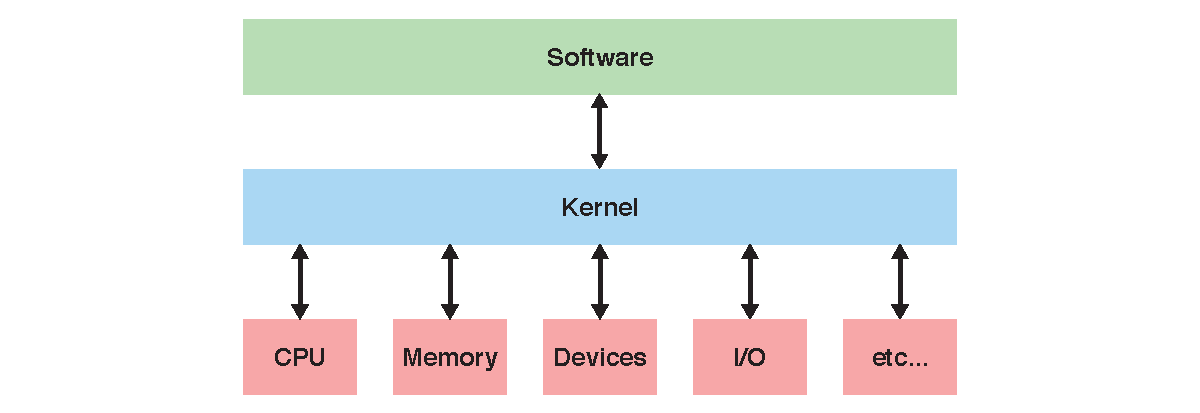
\includegraphics[width=\textwidth]{figures/kernel.pdf}
    \caption{An oversimplification of who the kernel interacts with the hardware and software}
    \label{fig:kernel_visualization}
\end{figure}

\subsection{Jetpack}
The \jx runs an operating system called \gls{jetlinux} which is built on the Linux Kernel \cite{JetsonLinux352023}.
This operating system is part of a software suite called \gls{jetpack} which also includes things \cuda drivers and multimedia \gls{api} \cite{nvidiaJetPackSDK2023}.
The hierarcy is visualized in Figure \ref{fig:jetpack_hierarchy}.

\subsection{Results from the \preproject}
During the \preproject \gls{pps} interrupts were enabled on the \jx by following a guide from Mateusz Sadowski \cite{sadowskiEnablingPPSJetson2020} \cite[26]{martensPortableSensorRig2022}.
Althogh the guide was written for \jetson Nano running \gls{jetpack} 4.3, it worked on the \jx running \gls{jetpack} 4.6 as well after minor modifications \cite{sadowskiEnablingPPSJetson2020} \cite[26]{martensPortableSensorRig2022}.
The \gls{deepstream} \gls{sdk} is used in the \master and requires the new version of \gls{jetpack}, 5.1, with CUDA 11.4 \cite{nvidiaDeepStreamSDKGet2019}.
The assumption was that it would not be more difficult to enable \gls{pps} on this version than it was with \gls{jetpack} 4.6.
This assumption turned out to be wrong, and the over all experience is vusialized in Figure \ref{fig:xkcd_cautionary}.

\subsection{Differences between current and previous version of \gls{jetpack}}
A significant difference between the two versions of \gls{jetpack} is that they are build on different versions of the Linux Kernel as well as file systems based on different version of Ubuntu \cite{nvidiaJetPackSDK2022} \cite{nvidiaJetPackSDK2023}.
The differences are visualized in Figure \ref{fig:jetpack_hierarchy}.
It is likely that the issues experienced when trying to compile the kernel are related to these major changes.
There might be some other root cause, but this remains unknown.

\begin{figure}[H]
    \centering
    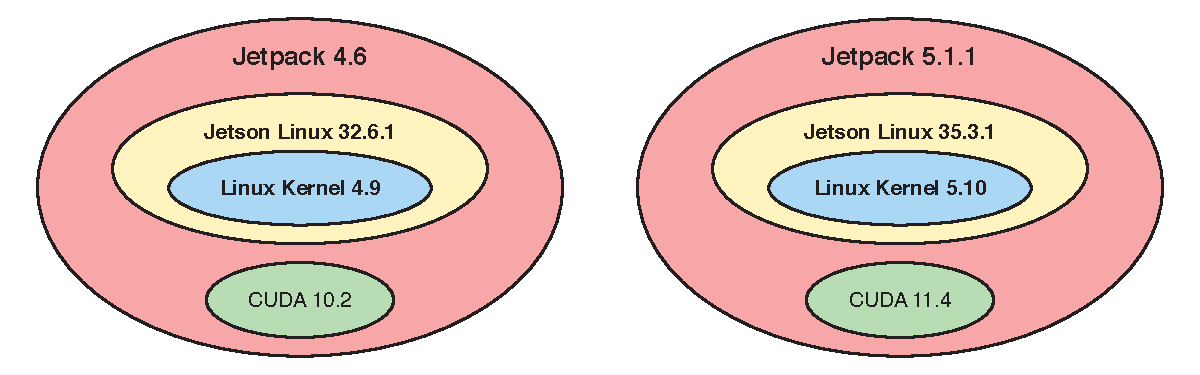
\includegraphics[width=\textwidth]{figures/jetpack_hierarchy/hierarchy.pdf}
    \caption{Visualization of the Jetpack hierarchy \cite{nvidiaJetPackSDK2022}\cite{nvidiaJetPackSDK2023}}
    \label{fig:jetpack_hierarchy}
\end{figure}

\subsection{Physical setup during compilation}
To flash the \jx it is necessary to have a host computer running Ubuntu \cite{nvidiaSDKManager2019}.
During the \preproject I attempted to flash the \jx using a docker image inside \gls{wsl} and communicationg with the \jx over usbipd-win, without success \cite{martensPortableSensorRig2022} \cite{nvidiaSDKManager2019} \cite{dorsselaerUsbipdwin2023}.
Since then people claim to have acheived this but I was not able to reproduce their result \jx \cite{makinbacon21TUTORIALUsingSdkmanager2022}.
Other posts on the forum appear to confirm my results \cite{2008PleaseProvideMore2022}.
It was possible however to build everything in a docker container on a windows computer, copy the files to a local computer and flashing the \jx from there,
but the time saved from using a more powerful computer did not outweigh the extra work needed to copy all the files.

Without the possibility to flash from a windows machine, the same spare laptop was used as during the \preproject, equiped with an Intel i7-7700HQ \gls{cpu} \cite{martensPortableSensorRig2022}.
The laptop was directly connected to the \jx using a usb-c cable.



\subsection{Initial attempts}
After discovering that the guide from Mateusz Sadowski not longer worked, a couple of days were spent trying out different suggestions from the \gls{nforum}, without any success \cite{martensPortableSensorRig2022}.
The process can be summarized in the following steps:
\begin{enumerate}
    \item Clean up the environment after the last failed attempt.
    \item Download and extrace everything through the JetPack \gls{sdk} Manager gui.
    \item Follow the first part of the guide from Mateusz Sadowski \cite{sadowskiEnablingPPSJetson2020}.
    \item Add some suggested modifications from the \gls{nforum}.
    \item Compile the kernel.
    \item Follow the second part of the guide from Mateusz Sadowski \cite{sadowskiEnablingPPSJetson2020}.
    \item Debug the result.
\end{enumerate}
The entire procedure lasted approximately three hours, during which most of the time was spent waiting.
It still consumed a significant amount work hours due to the need for regular human interaction, causing disruptions in the workflow on other tasks.
The negative impact of frequent context switching on productivity for software developers has been acknowledged and should be minimized if feasible \cite{meyerSoftwareDevelopersPerceptions2014}.
This became evident after several days of minimal tangible progress on this task or any other task.

\subsection{Challenges}
A challenging aspect of the development of the pipeline was that the compilation process had a tendency to fail silently.
Wrong environment variables, wrong file locations, wrong privileges, wrong compilation flags or wrong file contents would often not cause the pipeline to crash and throw an error.
Instead everything would appear normal and the errors would not be detected until the \jx gets stuck in some sort of boot loop after the whole process was complete, as shown in Figure \ref{fig:stuck_in_boot_loop}.

\begin{figure}[H]
    \centering
    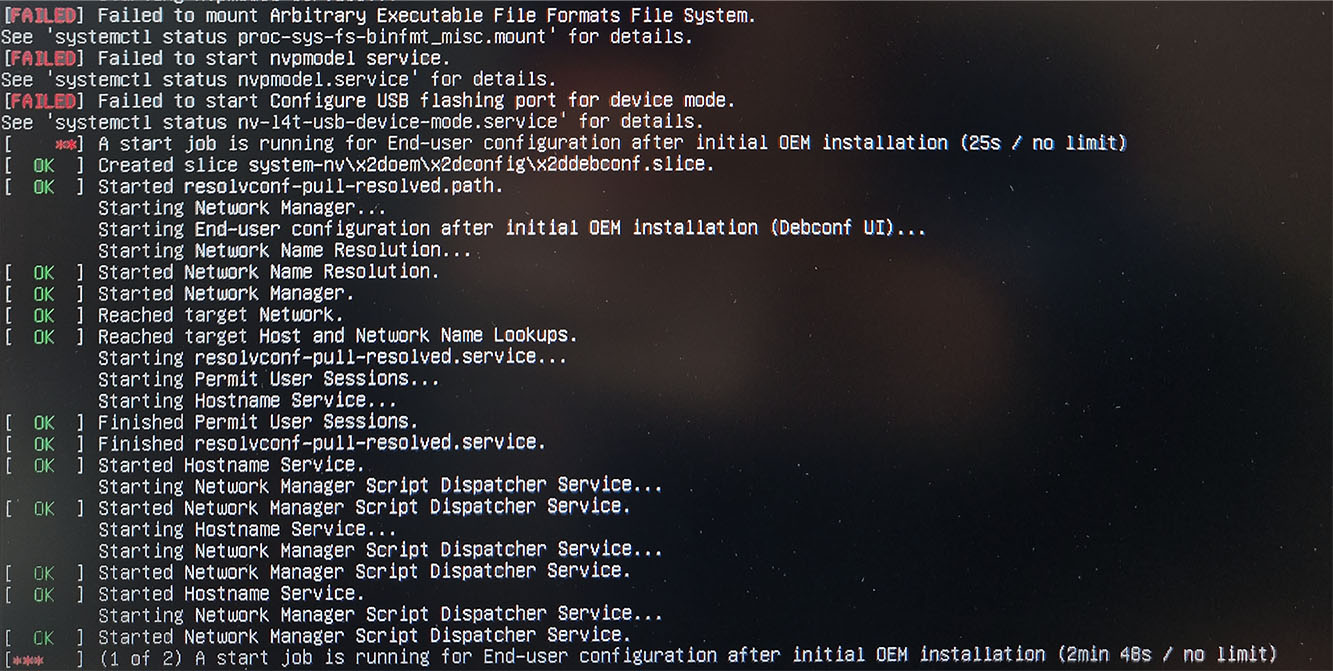
\includegraphics[width=1\textwidth]{figures/stuck_in_boot_loop.png}
    \caption{A recurring error when trying to flash the \jx}
    \label{fig:stuck_in_boot_loop}
\end{figure}

\subsection{Hesitation towards automation}
The main reason why the whole process was not automated from the begining was that it relied on using the graphical JetPack \gls{sdk} Manager to download and extract the necessary files to the right locations.
This took care of a lot obscure work that would otherwise have to be identified, but as it relied on a graphical interface it would not easy to integrate into any automation pipeline.
To fully automate the process it would be necessary to do all the work the \gls{sdk} Manager does, as well as the rest of the steps.

Still, after serveral days practically waisted on trying to get the process to work manually, it was decided to try to automate the entire process.
Another motivation for this was that learning how to flash a \jetson module properly seemed like a useful skill to aquire.

\subsection{Replacing the SDK Manager}
The first goal was to write a pipeline that could replace the visual \gls{sdk} Manager.
That is to write a pipaline capable of flashing the \jx with the latest unmodified version of \gls{jetlinux}.
This was harder than expected, as no documentation that takes you through the entire process was found.
Rather, different pieces of information scattered around on the different NVIDIA documents and on the \gls{nforum} were combined to get through the process.


\subsection{Removing all manual steps}
After having managed to flash the \jx with the latest unmodified version of \gls{jetlinux} it was time to improve the workflow.

After flashing the \jx it is normally necessary to connect the \jx to a monitor, keyboard and mouse, and manually create a user.
This is annyoing an time consuming but fortunately there was a script posted on the \gls{nforum} that can be used to automate this process \cite{waynewwwScriptBypassAccountJun2819}.

Another step that had to be done manually initially was to give the the user password to different processes to give them sudo persmission.
A simple solution to this was to use the followind code snippet:
\begin{minted}{bash}
    echo <password> | sudo -S <command>
\end{minted}
Doing this is of course not recommended as it is a security risk, but as a separate laptop was used for this task it was deemed acceptable in this particular case.

\subsection{Making the iteration speed faster}
As the compilation process took quite a while, it was important to make it as fast as possible to increase the iteration speed of the debugging process.
Firstly the compilation it self was also sped up by using all the cores on the computer.
Secondly the pipeline was designed to make it easy to have various checkpoints.
This removed the need to execute the whole process from start to end every time something went wrong.
For instance it was possible to cache the files that would be downloaded or skip the compilation step while development was done on the flashing process.
Lastly the \code{stderr} of every process was checked, which removed some of the silent failures.

\subsection{Gathering all manual steps}
The final goal in the automation process was to make it easy to include various modifications in the pipeline, so that different suggestions from the forums could be added implemented the beginning of the pipeline.
This was acheived by adding a new step in the pipeline that would copy modified files to given locations, and by making it easy to execute various defined shell commands at designated times.
This made it so that modifications and scipts could be defined ahead of the flashing, and the pipeline would add or execute them at the designated times, removing the need for any manual labour during the compilation and flashing process.
Writing autmated tests that could be executed over \gls{ssh} after flashing was concidered, but not consideret to be worth the time as different posts on the \gls{nforum} recommended checking different things.
Examples of this are searching for different keywords in the output from the \code{dmesg} command and checking the variables defined in \textit{/proc/config.gz}.

\subsection{Brute force solution}
After having replaced the \gls{sdk} Manager with a pipeline capable of flashing the \jx with modified version of
\gls{jetlinux} in an effieicnt and automated way, it was time to try to enable \gls{pps} interrupts.

The workflow now looked like this:
\begin{enumerate}
    \item Define modifications and scripts that would run during the compilation.
    \item Select checkpoint to start from.
    \item Run the pipeline.
    \item Debug the result.
\end{enumerate}

The final pipeline defines environment variables, executes 21 shell commands and modifies 3 of the source files.
With this workflow in place it was possible to test various suggestions from the \gls{nforum} in a more systematic way.
Having a profile on the \gls{nforum} was very useful, as it made it easy to filter out posts that I had already consulted when searching for solutions and bookmark the most relevant ones \cite{nvidiaNvidiaForumExtended2023}
As the all the manual steps were collected at the beginning or end of the process, it left up to two hours of uninterupted work time between each iteration that could be used to look for new suggesions or work on other tasks.

\subsection{Solution}
After days of using the new pipeline to try out different suggestions from the \gls{nforum} it was finally possible to enable \gls{pps} interrupts.
Goin into detail about all the different attempts that were made to enable \gls{pps} interrupts is beyond the scope of this thesis as 89 different forum posts from the \gls{nforum} with a total of 1092 replies, as well as several other blog posts and guides were consulted \cite{nvidiaNVIDIAJetsonLinux2023} \cite{nvidiaNVIDIATEGRALINUX} \cite{nvidiaNVIDIAJetsonLinux} \cite{nulizhuanzhuAGXXavier35} \cite{fishotterprojectEnablePpsSupport}.
The full list of relevant posts from the \gls{nforum} can be found in the appendix.
I also contacted and got response from a user on the \gls{nforum} who faced similar problems \cite{mhtechdevProgressPPS2023} and made a post that got relevant replies \cite{martensEnablePPSJetson2023}.
After solving my problems I posted my solution to contribute to the community \cite{martensEnablePPSJetson2023}.
The final key modifications are listed below.
\begin{itemize}
    \item Use Bootlin Toolchain gcc 9.3
    \item Modify the \textit{defconfig} file directly instead of the \textit{.config} file
    \item Make changes to the \code{pps_gpio_setup} function in \textit{pps-gpio.c}.
          % \item Set \code{CONFIG_PPS_DEBUG=y}
    \item Use \code{GPIO_ACTIVE_HIGH} not \code{GPIO_ACTIVE_LOW}
\end{itemize}





\subsection{Booting from SSD}
The non-cached read speed of the internal \gls{emmc} is significantly slower than the read speed of the \gls{ssd}.
This was evaluated using \code{hdparm}, a linux tool that can be used to test read spiied of a drive \cite{lordHdparmLinuxManual2018}.
The the folliwing two commands were run 3 times to get the average read speed of each device:
\begin{minted}{bash}
    sudo hdparm -Ttv /dev/mmcblk0 
    sudo hdparm -Ttv /dev/nvme0n1 
\end{minted}
With \gls{jetsonclocks} running and \gls{nvpmodel}=0, the buffered read speed of the \gls{emmc} is approximately 285MB while the buffered read speed of the \gls{ssd} is approximately 1010MB.
The built in \gls{emmc} also only has 32GB of storage \cite{nvidiaNVIDIAJetsonAGX2019} wich might be to small for the root partition in the future.

Based on this it was decided to write the \gls{jetlinux} to the Micron® 2300 SSD with NVMe™ 512GB \gls{ssd} and boot from there to increase performance \cite{microntechnologyMicron2300SSD2020}.
This was also challenging as a new flashing utility, called \code{intrid} was needed to acheive this \cite{rigerunNVIDIAJetpackFlashing2021}, and a compatible partitioning table had to be created \cite{nvidiaPartitionConfigurationJetson2022}.
Fortunately the established flashing pipeline made it considerably easier to aceive this than it would have been otherwise.

The performance difference between having the root partition on the \gls{emmc} and the \gls{ssd} remains to be evaluated properly.

\subsection{Reflections on the automation process}
The estimated cost and benefit of automation can often be very optimistic, as illustrated in Figure \ref{fig:xkcd_automation}.
It is not possible to know the effort it would have taken to find a working solution wihtout automating the process, but the current hypothesis is that the extra time spent on automation is equivalent to the time saved, if not slightly less.
If it was certain that this was the last time ever compiling an \jx, or a related \jetson product like the \jo, defending the time spent on automation would be hard.
However as this was a necessery part during the \preproject and remained necessary to repeat again here, it seems likely that this will not be the last time kernel configurations will be requiered in my work.
This is also supported by the fact that the \nvidia celebrated one million developers using the \nvidia \jetson platform, making it likely to remain a relevant platform in the foreseeable future \cite{blackNVIDIACelebratesMillion2023}.
Having this working pipeline will make future modifications easier, and also serve as a full pragmatic walkthrough  on how to modify, compile and flash a \jetson product.

\begin{figure}[H]
    \centering
    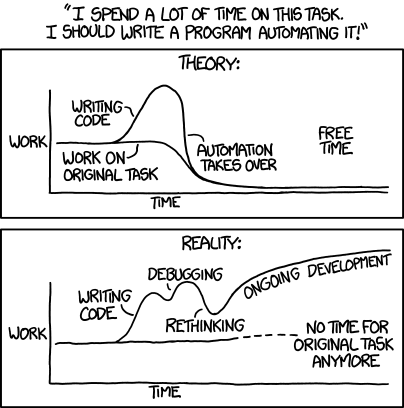
\includegraphics[width=0.5\textwidth]{figures/xkcd_automation.png}
    \caption{Automation by XKCD \cite{xkcdAutomation2014}}
    \label{fig:xkcd_automation}
\end{figure}

